\section{增广Lagrange法（ALM）}
\label{sec:pm-alm}

前面两条路各有缺陷。二次罚能增加法向曲率，把子问题变成好解的碗，但违规量要靠$\rho\to\infty$才能消失。对偶上升不增加任何曲率，步长稍大就振荡，目标线性时子问题甚至定不出解。把价格和罚款放在同一个函数里，能否在有限的$\rho$下得到解？

\paragraph{从力的平衡出发}
二次罚的驻点满足$\nabla f+\rho\bm{J}^\top\bm{h}=\bm{0}$。要平衡目标的力，$\rho\bm{h}$必须接近$\bm{\nu}^\star$，所以$\bm{h}$不能为零。如果事先在罚项里加上一个估计的力$\bm{\nu}$，那么只要$\bm{\nu}$足够接近$\bm{\nu}^\star$，弹簧几乎不用拉长。

工厂的语言是，总部既标出单价，又对偏离总量收罚款。单价负责提供大部分的调节力，罚款只负责修正单价还没估准的那一小部分。写成函数，就是在Lagrange函数上加残差平方。

\begin{definition}[增广Lagrange函数]
\label{def:pm-al}
对等式约束问题和$\rho>0$，\term{增广Lagrange函数}（augmented Lagrangian）是
\begin{equation}
 \mathcal{L}_\rho(\bm{x},\bm{\nu})=f(\bm{x})+\langle\bm{\nu},\bm{h}(\bm{x})\rangle+\frac{\rho}{2}\lVert\bm{h}(\bm{x})\rVert_2^2 .
 \label{eq:pm-al}
\end{equation}
\end{definition}

配方之后可以看出它的结构：
\begin{equation}
 \mathcal{L}_\rho(\bm{x},\bm{\nu})=f(\bm{x})+\frac{\rho}{2}\Bigl\lVert\bm{h}(\bm{x})+\frac{\bm{\nu}}{\rho}\Bigr\rVert_2^2-\frac{1}{2\rho}\lVert\bm{\nu}\rVert_2^2 .
 \label{eq:pm-al-square}
\end{equation}
最后一项与$\bm{x}$无关。所以固定$\bm{\nu}$时，增广Lagrange函数就是一个目标移位的二次罚：它不再要求$\bm{h}=\bm{0}$，而是把残差往$-\bm{\nu}/\rho$处拉。移位量选得对，平衡点上的残差就恰好是零。

\paragraph{同一个例子}
对二元例，固定$\nu$和$\rho$，增广Lagrange函数的驻定方程是
\[
 (1+\rho)x_1+\rho x_2=4\rho-\nu,\qquad \rho x_1+(3+\rho)x_2=4\rho-\nu .
\]
两式相减仍得$x_1=3x_2$。代回得到
\begin{equation}
 x_2=\frac{4\rho-\nu}{3+4\rho},\qquad x_1=3x_2 .
 \label{eq:pm-running-al-solution}
\end{equation}
残差因此是
\begin{equation}
 h(\bm{x})=4x_2-4=-\frac{4(\nu+3)}{3+4\rho}.
 \label{eq:pm-running-al-residual}
\end{equation}
和二次罚的式~\eqref{eq:pm-running-penalty-residual}比较，二次罚对应$\nu=0$，残差只能靠分母变大。这里分子含有因子$\nu-\nu^\star=\nu+3$：只要$\nu=-3$，无论$\rho$多小，残差都是零。

图~\ref{fig:pm-alm-center}固定$\rho=1.5$，只改变$\nu$。等高线的形状完全不变，因为Hessian不依赖$\nu$；变的是碗底的位置，$\nu=0$时离直线较远，$\nu=-2$时贴近直线，$\nu=-3$时恰好落在解上。对比图~\ref{fig:pm-penalty-contours}，那里要靠压扁碗才能靠近直线，这里碗的形状没有变。

\begin{BookInlineFigure}
  \centering
  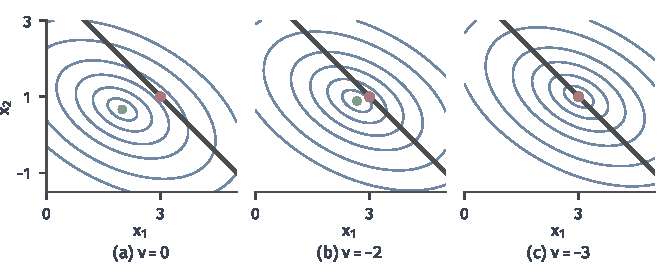
\includegraphics[width=112mm]{figures/05-optimization/06-constrained-optimization/matplotlib/pm-alm-center/figure.pdf}
  \caption{二元例中$\mathcal{L}_{1.5}(\cdot,\nu)$的等高线（蓝），$\rho=1.5$固定。深灰直线是约束，绿点是增广函数的最小点，红点是解$(3,1)$。改变乘子只平移碗底，不改变碗的形状；(c)$\nu=\nu^\star$时最小点落在解上。}
  \label{fig:pm-alm-center}
\end{BookInlineFigure}

这种现象不只在二次例子里出现，它在局部有一般的解释。下面的定理说，只要乘子是对的，有限的$\rho$就够了。

\begin{theorem}[最优乘子下的局部精确性]
\label{thm:pm-al-exact}
设$f,h_j$二阶连续可微，$(\bm{x}^\star,\bm{\nu}^\star)$满足KKT条件。记$\bm{W}$为$\mathcal{L}(\cdot,\bm{\nu}^\star)$在$\bm{x}^\star$处的Hessian，$\bm{J}=\bm{J}(\bm{x}^\star)$，并设对所有非零$\bm{d}$，只要$\bm{J}\bm{d}=\bm{0}$，就有$\bm{d}^\top\bm{W}\bm{d}>0$。则存在$\bar\rho\geq0$，使$\rho>\bar\rho$时，$\bm{x}^\star$是$\mathcal{L}_\rho(\cdot,\bm{\nu}^\star)$的严格局部最小点。
\end{theorem}

\begin{proof}
由$\bm{h}(\bm{x}^\star)=\bm{0}$和KKT条件，
\[
 \nabla_{\bm{x}}\mathcal{L}_\rho(\bm{x}^\star,\bm{\nu}^\star)=\nabla f+\bm{J}^\top\bm{\nu}^\star+\rho\bm{J}^\top\bm{h}=\bm{0}.
\]
含$h_j\nabla^2h_j$的项在$\bm{x}^\star$处为零，所以Hessian是
\[
 \nabla^2_{\bm{x}\bm{x}}\mathcal{L}_\rho(\bm{x}^\star,\bm{\nu}^\star)=\bm{W}+\rho\bm{J}^\top\bm{J}.
\]
只需证明$\rho$足够大时它正定。$\bm{J}^\top\bm{J}$半正定，这个矩阵关于$\rho$是单调的，一旦正定，更大的$\rho$也正定。

用反证法。若对每个正整数$k$，$\bm{W}+k\bm{J}^\top\bm{J}$都不正定，则存在单位向量$\bm{u}_k$，使
\[
 \bm{u}_k^\top\bm{W}\bm{u}_k+k\lVert\bm{J}\bm{u}_k\rVert_2^2\leq0 .
\]
单位向量的序列有收敛子列，设极限为$\bm{u}$。由上式得
\[
 \lVert\bm{J}\bm{u}_k\rVert_2^2\leq\frac{\lVert\bm{W}\rVert_2}{k}\to0 ,
\]
故$\bm{J}\bm{u}=\bm{0}$。

不等式的第二项非负，去掉它得$\bm{u}_k^\top\bm{W}\bm{u}_k\leq0$，取极限得$\bm{u}^\top\bm{W}\bm{u}\leq0$。这与假设矛盾，因为$\bm{u}\neq\bm{0}$且$\bm{J}\bm{u}=\bm{0}$。
\end{proof}

条件中$\bar\rho$的作用，看一个非凸的例子。取$f(\bm{x})=\tfrac12(x_1^2-x_2^2)$，$h(\bm{x})=x_2$，解是原点，$\nu^\star=0$。切方向是$x_1$轴，曲率$1>0$，满足二阶条件。此时增广函数的Hessian是$\operatorname{diag}(1,\rho-1)$，必须$\rho>1$才正定。$\rho<1$时，增广函数沿$x_2$方向没有下界。若$f$是凸函数且约束是线性的，就不需要这个门槛，任何$\rho>0$都行。

\subsection{原始变量与乘子更新}
\label{sec:pm-alm-update}

问题转到怎样得到正确的乘子。上一节的定理给了线索：用$\bm{\nu}$算出的增广函数的驻点，本身就告诉我们乘子该往哪里改。

\paragraph{主要思想}
对$\mathcal{L}_\rho$求梯度，把含$\bm{h}$的项合并，得到一个恒等式：
\begin{equation}
 \nabla_{\bm{x}}\mathcal{L}_\rho(\bm{x},\bm{\nu})=\nabla f(\bm{x})+\bm{J}(\bm{x})^\top\bigl(\bm{\nu}+\rho\bm{h}(\bm{x})\bigr)=\nabla_{\bm{x}}\mathcal{L}\bigl(\bm{x},\bm{\nu}+\rho\bm{h}(\bm{x})\bigr).
 \label{eq:pm-al-gradient-identity}
\end{equation}
如果$\bm{x}^{(t+1)}$是增广函数的驻点，那么它对应的Lagrange函数在乘子$\bm{\nu}^{(t)}+\rho\bm{h}(\bm{x}^{(t+1)})$处驻定。这个乘子把目标的力和约束的力平衡起来了，正好作为新的估计。

由此得到\term{增广Lagrange法}（augmented Lagrangian method，ALM）：
\begin{equation}
 \begin{aligned}
 \bm{x}^{(t+1)}&\approx\argmin_{\bm{x}}\mathcal{L}_{\rho}(\bm{x},\bm{\nu}^{(t)}),\\
 \bm{\nu}^{(t+1)}&=\bm{\nu}^{(t)}+\rho\,\bm{h}(\bm{x}^{(t+1)}).
 \end{aligned}
 \label{eq:pm-alm}
\end{equation}
这里$\rho$既是罚参数，也是乘子的步长。把步长取成$\rho$，正是恒等式~\eqref{eq:pm-al-gradient-identity}选出来的，不是任意的约定。

形式上它和对偶上升~\eqref{eq:pm-dual-ascent}只差一点：残差的取法。对偶上升先在旧乘子下解Lagrange子问题，用得到的残差算新乘子。ALM的$\bm{x}^{(t+1)}$满足的是新乘子下的驻定条件，残差实际上是在“走到之后的乘子”处读的。这正是第~\ref{chap:nonsmooth-composite-optimization}章显式步和隐式步的区别。

\begin{theorem}[ALM是对偶问题的邻近点法]
\label{thm:pm-alm-proximal}
设$f$是适当、闭的凸函数，$\bm{h}(\bm{x})=\bm{A}\bm{x}-\bm{b}$。设$\bm{x}^{+}$是$\mathcal{L}_\rho(\cdot,\bm{\nu})$的全局最小点，$\bm{\nu}^{+}=\bm{\nu}+\rho\bm{h}(\bm{x}^{+})$。则$\bm{x}^{+}$是$\mathcal{L}(\cdot,\bm{\nu}^{+})$的全局最小点，并且
\begin{equation}
 \bm{\nu}^{+}=\bm{\nu}+\rho\bm{s}^{+},\qquad \bm{s}^{+}=\bm{h}(\bm{x}^{+})\text{是}q\text{在}\bm{\nu}^{+}\text{处的超梯度},
 \label{eq:pm-alm-implicit}
\end{equation}
等价地，$\bm{\nu}^{+}$是下面问题的唯一解：
\begin{equation}
 \bm{\nu}^{+}=\argmax_{\bm{y}}\Bigl\{q(\bm{y})-\frac{1}{2\rho}\lVert\bm{y}-\bm{\nu}\rVert_2^2\Bigr\}.
 \label{eq:pm-alm-prox}
\end{equation}
\end{theorem}

\begin{proof}
$\bm{x}^{+}$最小化凸函数$\mathcal{L}_\rho(\cdot,\bm{\nu})$，最优性条件是
\[
 \bm{0}\in\partial f(\bm{x}^{+})+\bm{A}^\top\bigl(\bm{\nu}+\rho(\bm{A}\bm{x}^{+}-\bm{b})\bigr)=\partial f(\bm{x}^{+})+\bm{A}^\top\bm{\nu}^{+}.
\]
这正是凸函数$\mathcal{L}(\cdot,\bm{\nu}^{+})$在$\bm{x}^{+}$处的最优性条件，第一个结论成立。

由定理~\ref{thm:pm-residual-supergradient}，$\bm{s}^{+}=\bm{h}(\bm{x}^{+})$是$q$在$\bm{\nu}^{+}$处的超梯度，再由$\bm{\nu}^{+}$的定义得式~\eqref{eq:pm-alm-implicit}。

式~\eqref{eq:pm-alm-prox}中的目标强凹。它在$\bm{\nu}^{+}$处的最优性条件是$\bm{0}$属于$\partial q(\bm{\nu}^{+})-(\bm{\nu}^{+}-\bm{\nu})/\rho$，而式~\eqref{eq:pm-alm-implicit}正好给出这样一个超梯度。
\end{proof}

图~\ref{fig:pm-explicit-implicit}在二元例上比较两种步。$\rho=1.5$，从$\nu^{(0)}=0$出发，$q$的斜率是$-4$。显式步用当前点的斜率，走到$0+1.5\times(-4)=-6$，越过最大点，这就是图~\ref{fig:pm-dual-ascent}(b)的振荡。隐式步要求落点的斜率$s$满足$\nu^{+}=\nu+1.5s$，代入$s=-\tfrac43\nu^{+}-4$，解出$\nu^{+}=-2$，落在最大点的同一侧。

\begin{BookInlineFigure}
  \centering
  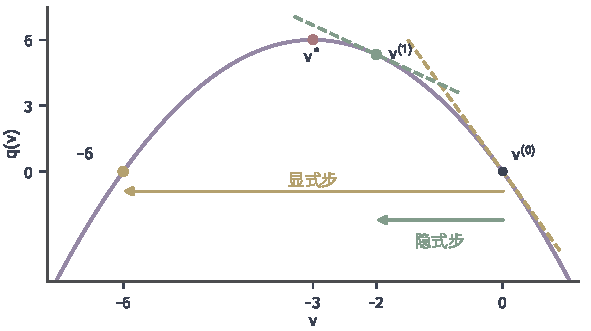
\includegraphics[width=100mm]{figures/05-optimization/06-constrained-optimization/matplotlib/pm-explicit-implicit/figure.pdf}
  \caption{同样的步长$\rho=1.5$下，对偶函数（紫）上的显式步与隐式步。黄色虚线是$\nu^{(0)}=0$处的切线，显式步按它的斜率走到$-6$（黄点）。绿色虚线是$\nu^{(1)}=-2$处的切线，隐式步要求落点切线的斜率与步长一致，得到绿点。红点是最大点$\nu^\star$。}
  \label{fig:pm-explicit-implicit}
\end{BookInlineFigure}

\begin{BookInlineTable}
  \centering
  \begin{tabular}{@{}lll@{}}
    \toprule
     & 对偶上升 & ALM\\
    \midrule
    原始子问题 & $\min\mathcal{L}(\cdot,\bm{\nu})$ & $\min\mathcal{L}_\rho(\cdot,\bm{\nu})$\\
    残差读取点 & 旧乘子（显式） & 新乘子（隐式）\\
    步长限制 & 受$q$的曲率限制 & 任意$\rho>0$（凸问题）\\
    子问题 & 目标可分则可分 & 平方项通常耦合各块\\
    目标线性时 & 子问题可能无解或解不唯一 & 平方项提供曲率\\
    \bottomrule
  \end{tabular}
  \caption{对偶上升与ALM的对照。ALM用更难的子问题换取稳定的乘子更新。}
  \label{tab:pm-dual-vs-alm}
\end{BookInlineTable}

压缩的速度可以显式写出。下面的定理针对最简单的等式约束二次规划，它的结论和图上的行为完全一致。

\begin{theorem}[线性等式二次问题的压缩率]
\label{thm:pm-alm-quadratic-rate}
设$f$是二次函数$\tfrac12\bm{x}^\top\bm{G}\bm{x}-\bm{d}^\top\bm{x}$，$\bm{G}\succ\bm{0}$，$\bm{h}(\bm{x})=\bm{A}\bm{x}-\bm{b}$，$\bm{A}$行满秩，记$\bm{S}=\bm{A}\bm{G}^{-1}\bm{A}^\top$。则精确求解子问题的ALM满足
\begin{equation}
 \bm{\nu}^{(t+1)}-\bm{\nu}^\star=(\bm{I}+\rho\bm{S})^{-1}(\bm{\nu}^{(t)}-\bm{\nu}^\star),
 \label{eq:pm-alm-linear-map}
\end{equation}
于是
\begin{equation}
 \lVert\bm{\nu}^{(t+1)}-\bm{\nu}^\star\rVert_2\leq\frac{1}{1+\rho\,\lambda_{\min}(\bm{S})}\lVert\bm{\nu}^{(t)}-\bm{\nu}^\star\rVert_2 .
 \label{eq:pm-alm-rate}
\end{equation}
\end{theorem}

\begin{proof}
由恒等式~\eqref{eq:pm-al-gradient-identity}，$\bm{x}^{(t+1)}$满足
\[
 \bm{G}\bm{x}^{(t+1)}-\bm{d}+\bm{A}^\top\bm{\nu}^{(t+1)}=\bm{0},
\]
解出
\[
 \bm{x}^{(t+1)}=\bm{G}^{-1}(\bm{d}-\bm{A}^\top\bm{\nu}^{(t+1)}).
\]
代入乘子更新式，得到
\[
 \bm{\nu}^{(t+1)}-\bm{\nu}^{(t)}=\rho\bigl(\bm{A}\bm{G}^{-1}\bm{d}-\bm{S}\bm{\nu}^{(t+1)}-\bm{b}\bigr).
\]
$\bm{\nu}^\star$满足同样形式的方程
\[
 \bm{A}\bm{G}^{-1}\bm{d}-\bm{S}\bm{\nu}^\star-\bm{b}=\bm{0},
\]
两式相减，得到
\[
 \bm{\nu}^{(t+1)}-\bm{\nu}^{(t)}=-\rho\bm{S}(\bm{\nu}^{(t+1)}-\bm{\nu}^\star).
\]
移项得
\[
 (\bm{I}+\rho\bm{S})(\bm{\nu}^{(t+1)}-\bm{\nu}^\star)=\bm{\nu}^{(t)}-\bm{\nu}^\star ,
\]
即式~\eqref{eq:pm-alm-linear-map}。$\bm{S}$对称正定，取范数即得式~\eqref{eq:pm-alm-rate}。
\end{proof}

二元例中$\bm{S}=1+\tfrac13=\tfrac43$，压缩因子是$3/(3+4\rho)$，$\rho=1.5$时为$\tfrac13$。任何$\rho>0$都是压缩的，和对偶上升要求$\alpha<\tfrac32$形成对比。

\paragraph{计算过程}
仍用二元例，并沿用第~\ref{sec:pm-rho-update}小节的外层容差。

\needspace{6\baselineskip}
\paragraph{变量}
\begin{itemize}
 \item $\bm{\nu}^{(t)}\in\mathbb{R}^p$：乘子估计。例中$p=1$。
 \item $\bm{x}^{(t)}\in\mathbb{R}^n$：增广子问题的解。例中$n=2$。
 \item $\rho>0$：罚参数，下一小节讨论它的调整。
\end{itemize}

\paragraph{初始化}
取$\bm{\nu}^{(0)}$和$\rho$。例中$\nu^{(0)}=0$，$\rho=1.5$，外层容差$\varepsilon=0.05$。

\needspace{6\baselineskip}
\paragraph{每轮更新}
\begin{enumerate}
 \item 近似最小化$\mathcal{L}_\rho(\cdot,\bm{\nu}^{(t)})$。例中由式~\eqref{eq:pm-running-al-solution}，$\rho=1.5$时$x_2=(6-\nu)/9$，第一轮
 \[
  \bm{x}^{(1)}=\Bigl(2,\ \frac23\Bigr).
 \]
 \item 计算残差。例中第一轮
 \[
  h(\bm{x}^{(1)})=-\frac43 .
 \]
 \item 由式~\eqref{eq:pm-alm}更新乘子。例中第一轮
 \[
  \nu^{(1)}=0+1.5\times\Bigl(-\frac43\Bigr)=-2 .
 \]
\end{enumerate}
第二轮得到
\[
 \bm{x}^{(2)}=\Bigl(\frac83,\ \frac89\Bigr),\qquad h(\bm{x}^{(2)})=-\frac49,\qquad \nu^{(2)}=-\frac83 .
\]
第三轮得到
\[
 \bm{x}^{(3)}=\Bigl(\frac{26}{9},\ \frac{26}{27}\Bigr),\qquad h(\bm{x}^{(3)})=-\frac{4}{27},\qquad \nu^{(3)}=-\frac{26}{9}.
\]
第四轮得到
\[
 \bm{x}^{(4)}=\Bigl(\frac{80}{27},\ \frac{80}{81}\Bigr),\qquad h(\bm{x}^{(4)})=-\frac{4}{81}\approx-0.049 .
\]

结束条件是$\lvert h\rvert\leq\varepsilon$，例中第四轮满足。最终得到$\bm{x}^{(4)}\approx(2.963,0.988)$，更新后的乘子是$\nu^{(4)}=-\tfrac{80}{27}\approx-2.963$。

第一轮和二次罚$\rho=1.5$的结果相同，因为此时$\nu=0$。此后二次罚换$\rho$，ALM换$\nu$。用相同的梯度法作内层，四轮分别用$21$、$18$、$15$、$12$步，共$66$步，$\rho$一直是$1.5$，条件数一直是$3.1$。

图~\ref{fig:pm-alm-vs-penalty}(a)比较两种方法。按外层轮数看，二次罚（$\rho$每轮乘$10$）下降得更快；但它每一轮都在解一个更病态的问题。ALM每轮只把残差缩小到$\tfrac13$，却始终在解同一个条件数很小的问题。(b)是ALM中$\rho$的取舍：$\rho$越大，外层压缩因子越小，轮数越少，内层条件数越大。

\begin{BookInlineFigure}
  \centering
  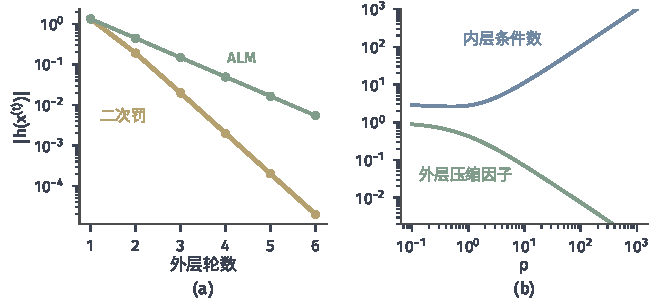
\includegraphics[width=112mm]{figures/05-optimization/06-constrained-optimization/matplotlib/pm-alm-vs-penalty/figure.pdf}
  \caption{二元例上ALM与二次罚的对比。(a)半对数坐标下的约束残差：黄线是二次罚（$\rho$从$1.5$开始每轮乘$10$），绿线是ALM（$\rho=1.5$固定），每轮精确求解。(b)双对数坐标，绿线是ALM的外层压缩因子$3/(3+4\rho)$，蓝线是内层Hessian的条件数。}
  \label{fig:pm-alm-vs-penalty}
\end{BookInlineFigure}

\paragraph{不等式约束}
前面的公式都是等式约束，不等式约束的乘子有符号限制，不能直接照搬。标准的做法是加入非负松弛变量，把$g_i(\bm{x})\leq0$写成$g_i(\bm{x})+s_i=0$，$s_i\geq0$，然后只对这个等式写增广函数。

固定$\bm{x}$，把$s_i$的优化解出来。对第$i$条约束，要在$s_i\geq0$上最小化
\[
 \lambda_i(g_i+s_i)+\frac\rho2(g_i+s_i)^2 .
\]
这是$s_i$的凸二次函数，无约束极小点是$-g_i-\lambda_i/\rho$，投影到非负数后得到
\[
 s_i=\Bigl[-g_i-\frac{\lambda_i}{\rho}\Bigr]_+ .
\]
由此可得$g_i+s_i=\max\{g_i,-\lambda_i/\rho\}$。把它代回去，分$g_i\geq-\lambda_i/\rho$和$g_i<-\lambda_i/\rho$两种情形合并，增广函数为
\begin{equation}
 \mathcal{L}_\rho(\bm{x},\bm{\lambda})=f(\bm{x})+\frac{1}{2\rho}\sum_{i=1}^m\Bigl([\lambda_i+\rho g_i(\bm{x})]_+^2-\lambda_i^2\Bigr).
 \label{eq:pm-al-inequality}
\end{equation}
乘子沿松弛等式更新，$\lambda_i^{+}=\lambda_i+\rho(g_i+s_i)$，整理后是
\begin{equation}
 \lambda_i^{+}=\bigl[\lambda_i+\rho g_i(\bm{x})\bigr]_+ .
 \label{eq:pm-alm-inequality-update}
\end{equation}

这个公式自动带来了对偶可行和互补。$\lambda_i^{+}$是正部，所以非负。若$g_i<-\lambda_i/\rho$，约束有足够余量，$\lambda_i^{+}=0$，该约束暂时不起作用。不动点$\lambda_i^{+}=\lambda_i$等价于$\max\{g_i,-\lambda_i/\rho\}=0$，它恰好是
\begin{equation}
 g_i\leq0,\qquad \lambda_i\geq0,\qquad \lambda_ig_i=0 .
 \label{eq:pm-complementarity}
\end{equation}
图~\ref{fig:pm-alm-ineq}(a)是单条约束的代价：在$g\geq-\lambda/\rho$一侧是二次增长的曲线，另一侧是常数$-\lambda^2/(2\rho)$，两段光滑相接。(b)是乘子更新，折线在$-\lambda/\rho$处把负值截断。

\begin{BookInlineFigure}
  \centering
  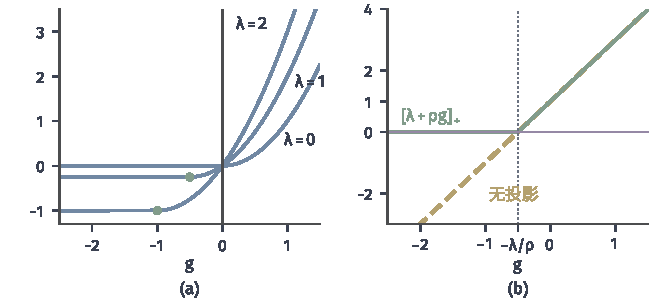
\includegraphics[width=112mm]{figures/05-optimization/06-constrained-optimization/matplotlib/pm-alm-ineq/figure.pdf}
  \caption{不等式约束的增广项，$\rho=2$。(a)蓝线是$([\lambda+\rho g]_+^2-\lambda^2)/(2\rho)$关于$g$的曲线，$\lambda=0,1,2$，绿点是分段点$g=-\lambda/\rho$，深灰竖线是约束边界。(b)$\lambda=1$的乘子更新：绿线是投影形式$[\lambda+\rho g]_+$，黄色虚线是不作投影的直线，紫线是零。}
  \label{fig:pm-alm-ineq}
\end{BookInlineFigure}

用一维例检验。式~\eqref{eq:pm-one-dim}的$g=1-x$，式~\eqref{eq:pm-al-inequality}对$x$的导数是
\[
 1-[\lambda+\rho(1-x)]_+ .
\]
令其为零，得到
\[
 x=1+\frac{\lambda-1}{\rho}.
\]
此时$\lambda+\rho(1-x)=1$，所以由式~\eqref{eq:pm-alm-inequality-update}，不管$\lambda$从哪里开始，一次更新后都有$\lambda^{+}=1=\lambda^\star$。第二轮代入，$x=1$，就是原问题的解。二次罚在同一例上永远差$1/\rho$。

不作投影会出错。考虑$\min x^2$，$x\geq-1$，解$x^\star=0$，约束不活动，$\lambda^\star=0$。写$g=-1-x$，取$\rho=2$，$\lambda^{(0)}=0$。式~\eqref{eq:pm-alm-inequality-update}给出$\lambda^{+}=0$，一步就对。

若把它当作等式，用不带投影的公式，子问题的解是$x=(\lambda-2)/4$，乘子递推是$\lambda^{+}=\tfrac12\lambda-1$。序列$\lambda=0,-1,-1.5,\ldots$趋于$-2$，$x$趋于$-1$。这是把约束当作$x=-1$时的解，既不是原问题的解，乘子的符号也错了。

\subsection{参数与停止条件}
\label{sec:pm-alm-parameters}

ALM的结构已经确定，剩下三件事：什么时候放大$\rho$，子问题解到多准，什么时候算结束。

\paragraph{罚参数}
不必让$\rho$趋于无穷，但也不能太小。$\rho$太小时，一方面非凸问题的子问题可能无下界，另一方面外层压缩很慢。常用的规则是观察约束残差是否下降到位。把等式残差和不等式残差放在同一个向量里：
\begin{equation}
 \bm{c}^{(t)}=\Bigl(\bm{h}(\bm{x}^{(t)}),\ \max\bigl\{\bm{g}(\bm{x}^{(t)}),-\bm{\lambda}^{(t-1)}/\rho^{(t-1)}\bigr\}\Bigr),
 \label{eq:pm-alm-residual-vector}
\end{equation}
其中$\max$按分量取。它把不活动约束的残差也按互补要求记为零。若
\begin{equation}
 \lVert\bm{c}^{(t+1)}\rVert_2>\theta\lVert\bm{c}^{(t)}\rVert_2,
 \label{eq:pm-alm-rho-test}
\end{equation}
说明残差下降不够，令$\rho\leftarrow\beta\rho$，否则保持$\rho$不变。常见取值是$\theta\in[0.25,0.5]$，$\beta\in[2,10]$。

顺序上，先用当前的$\rho$更新乘子，再放大$\rho$。乘子本身是一个不依赖$\rho$的量，放大$\rho$不需要换算它。

例如二元例若从$\rho=0.15$开始，压缩因子是$3/3.6\approx0.83$。第一轮和第二轮的结果为
\[
 h(\bm{x}^{(1)})=-\frac{10}{3},\qquad h(\bm{x}^{(2)})=-\frac{25}{9}.
\]
第二轮的残差比是$0.83$，大于$\theta=0.5$，所以把$\rho$放大到$1.5$，此后压缩因子变成$\tfrac13$。

\paragraph{内层精度}
恒等式~\eqref{eq:pm-al-gradient-identity}给出了一个便利之处：增广函数的内层梯度$\lVert\nabla_{\bm{x}}\mathcal{L}_\rho(\bm{x},\bm{\nu}^{(t)})\rVert_2$，正是更新后的乘子下Lagrange驻定残差。所以内层容差就是外层驻定精度，不用另算。

外层初期乘子还不准，把子问题解得太细是浪费。常用的安排是让内层容差$\omega^{(t)}$随外层逐步收紧，最终降到所需的驻定精度。对凸问题，邻近点法的分析要求内层误差可和，$\sum_t\epsilon^{(t)}<\infty$；实现上也常用与约束残差挂钩的相对准则。

\paragraph{三类残差}
结束时要分别检查三项，任何一项不合格都不算解好：
\begin{equation}
 \begin{aligned}
 \text{原始可行：}\quad&\lVert\bm{h}(\bm{x})\rVert_2,\ \ \lVert[\bm{g}(\bm{x})]_+\rVert_2\leq\varepsilon_{\mathrm{p}},\\
 \text{Lagrange驻定：}\quad&\lVert\nabla_{\bm{x}}\mathcal{L}(\bm{x},\bm{\lambda}^{+},\bm{\nu}^{+})\rVert_2\leq\varepsilon_{\mathrm{d}},\\
 \text{互补：}\quad&\lVert\min\{-\bm{g}(\bm{x}),\bm{\lambda}^{+}\}\rVert_2\leq\varepsilon_{\mathrm{c}}.
 \end{aligned}
 \label{eq:pm-alm-stopping}
\end{equation}
其中$\min$按分量取，它为零当且仅当式~\eqref{eq:pm-complementarity}成立。式中的第二项对应恒等式~\eqref{eq:pm-al-gradient-identity}，第一项不会因为内层解得准而自动变小，这一点和二次罚相同。

\paragraph{能保证什么}
ALM的保证分成三个层次，所需条件依次不同。先证明凸问题的情形，证明本身也说明了$\rho$为什么影响外层。

\begin{theorem}[凸问题的固定参数收敛]
\label{thm:pm-alm-convex}
设$f$是适当、闭的凸函数，$\bm{h}(\bm{x})=\bm{A}\bm{x}-\bm{b}$，存在最优解和最优乘子$\bm{\nu}^\star$，且强对偶成立。设$\rho>0$固定，各子问题的全局最小点存在且精确求解，$\bm{s}^{(t)}=\bm{h}(\bm{x}^{(t)})$。则
\begin{equation}
 \sum_{t\geq1}\rho^2\lVert\bm{s}^{(t)}\rVert_2^2\leq\lVert\bm{\nu}^{(0)}-\bm{\nu}^\star\rVert_2^2,
 \label{eq:pm-alm-summable}
\end{equation}
并且$\bm{h}(\bm{x}^{(t)})\to\bm{0}$，$q(\bm{\nu}^{(t)})\to d^\star$，$f(\bm{x}^{(t)})\to f^\star$。
\end{theorem}

\begin{proof}
记$\bm{\nu}=\bm{\nu}^{(t-1)}$，$\bm{\nu}^{+}=\bm{\nu}^{(t)}$，$\bm{s}^{+}=\bm{s}^{(t)}$。由定理~\ref{thm:pm-alm-proximal}，$\bm{s}^{+}$是$q$在$\bm{\nu}^{+}$处的超梯度。在式~\eqref{eq:pm-supergradient}中取比较点$\bm{\nu}^\star$，得到
\[
 q(\bm{\nu}^\star)\leq q(\bm{\nu}^{+})+\langle\bm{s}^{+},\bm{\nu}^\star-\bm{\nu}^{+}\rangle .
\]
$\bm{\nu}^\star$是$q$的最大点，所以$q(\bm{\nu}^{+})\leq q(\bm{\nu}^\star)$，上式给出
\[
 \langle\bm{s}^{+},\bm{\nu}^{+}-\bm{\nu}^\star\rangle\leq0 .
\]
现在把$\bm{\nu}=\bm{\nu}^{+}-\rho\bm{s}^{+}$代入$\lVert\bm{\nu}-\bm{\nu}^\star\rVert_2^2$并展开：
\[
 \lVert\bm{\nu}-\bm{\nu}^\star\rVert_2^2=\lVert\bm{\nu}^{+}-\bm{\nu}^\star\rVert_2^2-2\rho\langle\bm{s}^{+},\bm{\nu}^{+}-\bm{\nu}^\star\rangle+\rho^2\lVert\bm{s}^{+}\rVert_2^2 .
\]
中间项非负，舍去后得到
\[
 \lVert\bm{\nu}^{+}-\bm{\nu}^\star\rVert_2^2+\rho^2\lVert\bm{s}^{+}\rVert_2^2\leq\lVert\bm{\nu}-\bm{\nu}^\star\rVert_2^2 .
\]
对$t$求和裂项，即得式~\eqref{eq:pm-alm-summable}，于是$\bm{s}^{(t)}\to\bm{0}$，且$\bm{\nu}^{(t)}$有界。

再由第一个不等式，
\[
 0\leq d^\star-q(\bm{\nu}^{+})\leq\langle\bm{s}^{+},\bm{\nu}^\star-\bm{\nu}^{+}\rangle\leq\lVert\bm{s}^{+}\rVert_2\lVert\bm{\nu}^\star-\bm{\nu}^{+}\rVert_2\to0 .
\]
最后，由定理~\ref{thm:pm-alm-proximal}，$\bm{x}^{(t)}$是$\mathcal{L}(\cdot,\bm{\nu}^{(t)})$的全局最小点，所以
\[
 f(\bm{x}^{(t)})=q(\bm{\nu}^{(t)})-\langle\bm{\nu}^{(t)},\bm{s}^{(t)}\rangle ,
\]
右边趋于$d^\star=f^\star$。
\end{proof}

式~\eqref{eq:pm-alm-summable}中的$\rho^2$说明，$\rho$越大，残差平方的总和越小，外层越快。定理既不要求$\rho$放大，也不要求$f$可微，并且$\bm{x}^{(t)}$本身不一定收敛，$f$不强凸时子问题的解可以不唯一。

非凸问题只有局部结论。设$(\bm{x}^\star,\bm{\nu}^\star)$满足KKT条件，LICQ和二阶充分条件成立。那么存在$\bar\rho$，当$\rho\geq\bar\rho$时，从足够接近$\bm{\nu}^\star$的乘子出发，取$\mathcal{L}_\rho$在$\bm{x}^\star$附近的局部最小点，乘子序列线性收敛到$\bm{\nu}^\star$，压缩因子约为$O(1/\rho)$。这一结论的证明需要对驻定方程应用隐函数定理，篇幅较长，读者可查阅Nocedal和Wright的著作\scite{math-nocedal2006numerical}，它的机制和式~\eqref{eq:pm-alm-rate}相同。

全局层次的结果最弱。若每个子问题只解到近似驻点，乘子保持有界（常把估计截断在一个大盒子里），可以证明聚点要么是约束违规量的驻点，要么在相应约束资格下是KKT点；和定理~\ref{thm:pm-quadratic-approximate}的结论是同一类型。只有每个子问题都取全局最小点，才能得到全局最优的结论，非凸问题通常做不到。下表把三个层次放在一起。

\begin{BookInlineTable}
  \centering
  \small
  \begin{tabular}{@{}lll@{}}
    \toprule
    情形 & 主要条件 & 结论\\
    \midrule
    凸，固定$\rho$ & 强对偶，子问题精确 & 残差趋零，目标值收敛\\
    非凸，局部 & LICQ，二阶充分，$\rho\geq\bar\rho$ & 乘子局部线性收敛\\
    非凸，全局策略 & 近似驻点，乘子有界 & 聚点为不可行驻点或KKT点\\
    \bottomrule
  \end{tabular}
  \caption{ALM的三层保证。下面一行不能推出上面两行的结论。}
  \label{tab:pm-alm-guarantees}
\end{BookInlineTable}
